\documentclass{article}
%добавляет русский язык
\usepackage[english,russian]{babel}
\usepackage[14pt]{extsizes}
%Рисунки
\usepackage[dvips]{graphicx}
%Каталоги для рисунков

\graphicspath{{./image-parallel/}{image-git/}}
%Пакет работы с цветом
\usepackage{color}
%Пакет работы с гиперссылками и установка цвета ссылок
\usepackage[colorlinks,linkcolor=blue,urlcolor=blue]{hyperref}
%%TODO Настроить отступы 
%Добавление абзацев после оглавления (indentfirst)
\usepackage[indentfirst]{titlesec}
\usepackage{titletoc}
%%TODO Настроить нумерацию
\usepackage[utf8]{inputenc}
\linespread{1.3}
\author{Морозов С.Д.}
\begin{document}
\begin{titlepage}
	\centering
	{\LARGE Университет ИТМО \par}
	\vspace{5mm}
	{\Large Кафедра вычислительной техники\par}
	\vspace{1.5cm}
	{\huge\bfseries Отчет по прохождению практики\par}
	\vspace{3cm}
	\begin{flushleft}
		\hangindent=10cm
		\hangafter=-5
		\noindent 
		{\Large Студента\\
				P3311 группы \\
				Морозова С.Д.\\
				Руководитель \\
				Соснин В.В.
		}
	\end{flushleft}
	\vfill
% Bottom of the page
	\vspace{1cm}
	{\large Санкт-Петербург \par}
	{\large 2016  \par}
\end{titlepage}
%Нужны ли в содержании subsubsection'ы?
	\setcounter{tocdepth}{3}	
	\tableofcontents
	\newpage
	\section{Введение}
	\indent 
	%%Тема паралельные вычисления. Перед тем как приступить к тебе необходимо разобраться с латех и гит...
		Тема прохождения практики "--- параллельные вычисления. Цель задания "--- сравнить различные функции в языке С, которые 		можно использовать для измерения времени работы параллельных программ.
		
		Однако требования руководителя практики таковы, что перед тем как приступить к выполнению основного задания нужно 				ознакомиться с системой компьютерной вёрстки TeX (LaTeX), которая должна
	использоваться для написания отчёта, и ознакомиться с системой контроля версий Git, с последующим созданием учетной записи на 	сайте GitHub или анагичном.
	\newpage
	\section{Система компьютерной верстки \TeX(\LaTeX)}	
		\subsection{Краткое описание}
			\TeX ~"--- система компьютерной вёрстки с формулами, разработанная американским профессором информатики Дональдом 				Кнутом. Название происходит от греческого слова $\tau\varepsilon\chi\upsilon\eta$ "--- "<искусство">, "<мастерство">, 				поэтому	последняя буква читается как русская Х. Хотя TeX является системой набора и верстки, развитые возможности 					макроязыка TeX делают его Тьюринг-полным языком программирования. 
		
			\TeX ~работает с боксами (box) и клеем (glue). Бокс "--- двумерный объект прямоугольной формы, характеризуется тремя 
		величинами (высота, ширина, глубина). Элементарные боксы "--- это буквы, которые объединяются в боксы-слова, которые в 				свою очередь сливаются в боксы-строчки, боксы-абзацы и т.д.

        	Между боксами располагается клей, который имеет некоторую ширину по умолчанию и степени увеличения/уменьшения этой 				ширины. Объединяясь в бокс более высокого порядка, боксы могут шевелиться, но после того как найдено оптимальное решение, 		это состояние закрепляется, и полученный бокс выступает как единое целое.
        
       		Инетересный факт. На версии 3.0 дизайн был заморожен, поэтому в новых версиях не будет добавления новой 						функциональности, только исправление ошибок. Версия \TeX 'a ассимтотически приближается к числу $\pi$. Это факт говорит о 		том, что последняя версия	3.14159265 (январь 2014) является крайне стабильной и возможны лишь мелькие исправления. 				Дональд Кнут заявил, что последнее обновление (сделанное после его смерти) сменит номер версии на ~$\pi$, и с этого 				момента все ошибки станут особенностями.
        		
			\LaTeX ~"--- созданный Лесли Лэмпортом набор макрорасширений (или макропакет) системы компьютерной вёрстки \TeX, 				который облегчает набор сложных документов. Стоит отметить, что как и любой другой макропакет\footnote{ Так же существуют 		Plain TeX, AMS-TeX, AMS-LaTeX и т.д.} \LaTeX ~не может расширить возможности \TeX ~(все, что можно сделать в одном пакете 		можно сделать и в любом другом). Пакет позволяет автоматизировать многие задачи набора текста и подготовки статей, 					включая набор текста на нескольких языках, нумерацию разделов и формул, размещение иллюстраций и таблиц на странице, 				ведение библиографии и др. Все это делает \LaTeX ~крайне удобным инструментом для написания научных статей, диссертаций и 		т.п..
		\newpage
			
		\subsection{Сравнение \LaTeX ~и MS Word}
			В качестве сравнения "--- перечислим плюсы и минусы \LaTeX ~перед MS Word(а так же всеми его аналогами). \\	
	    Плюсы \LaTeX: 
	    \begin{itemize} 
	    	%\item	Проста работы с любыми математическими формулами
	    	\item	Кроссплатформенность 
	    	%\item	Без особых трудностей можно получить сноски, список литературы,
			%		оглавление, список таблиц, указатель и т. п.
	    	%\item	Имеется несколько стандартных стилей (книга, статья, доклад,
			%		письмо), с помощью которых получаются документы очень высокого
			%		полиграфического качества 
	    	%\item	Гибкая работа с логической структурой текста
	    	\item	Язык международного обмена по математике и физике (большинство     
   					научных издательств принимают тексты в печать  только в этом формате)
    	\end{itemize}
    	\newpage
    	Минусы \LaTeX:
		\begin{itemize} 
	    	\item	Не является системой типа WYSIWYG
	    				\footnote{What You See Is What You Get(Что видишь, то и получишь). Стоит отметить, что существуют 									дистрибутивы \TeX ~в которых есть попытки реализовать WYSIWYG. Например платный дистрибутив  BaKoMa TeX + 						текстовый редактор  BaKoMa TeX Word.}   
	    	\item	При серьезных отклонениях от стандартных стилей документов требуется
					достаточно сложное программирование	
    	\end{itemize}
    	
    		То есть, выбирая между \LaTeX ~и MS Word, стоит обратить внимание на то,какой текст вы собираетесь печатать, 					насколько нестандартный будет стиль текста, на его примерный объем. В некоторый случаях достаточно использовать MS Word,   		в других "--- использование \LaTeX ~может заметно упростить работу.
		\newpage		
		\subsection{Выбор инструмента редактирования}
			В ходе изучения всех возможных вариантов работа с \LaTeX ~для создания данного отчета, была выбрана программа 						Textmaker
			\footnote{Оффициальный сай Textmaker:~ \href{http://www.xm1math.net/texmaker/}{http://www.xm1math.net/texmaker/}}.\\
			Выбор Textmaker'а обусловлен следующими его особенностями:
			\begin{itemize} 
	    		\item	Автоматическая подсветка синтаксиса
	    		\item	Функция автодополнения команд \LaTeX
	    		\item	Сокрытие блоков кода (Code folding)
	    		\item	Быстрая навигация по структуре документа
	    		\item	Указание на строку с ошибкой, для быстрой отладки
	    		\item	Интегрированный просмотр PDF
			\end{itemize} 
	\newpage
	\section{Системы контроля версий}
		\subsection{Краткое описание}
			Система контроля версий (СКВ) — это система, регистрирующая изменения в одном или нескольких файлах с тем, чтобы в 				дальнейшем была возможность вернуться к определённым старым версиям этих файлов. 
				
			СКВ широко используются при разработке программного обеспечения, для хранения кодов разрабатываемых программ. Однако 			данные системы подходят не только программистам. Художники, которые хотят сохранять каждое изображение/эксиз своей 					работы, писатели пишущие книги или научные статьи, бухгалтеры, которые хранять разные версии отчетов и т.д., все они 				могут использовать СКВ для достижения своих целей.
				
			Иначе говоря СКВ можно применять в любых областях в которых ведётся работа с большим количеством непрерывно 					изменяющихся электронных документов.
		\subsection{Git}
			Git "--- созданная Линусом Торвальдсом, распределенная система контроля версий.
			\subsubsection{Особенности}
			% По большей части взято от сюда -> https://git-scm.com . Позже может быть перепишу своими словами.  
				Одной из основных особенностей Git состоит в способе хранения данных. В принципе, большинство других систем 					хранит 	информацию как список изменений (патчей) для файлов. Эти системы (CVS, Subversion, Perforce, Bazaar и другие) 			относятся к хранимым данным как к набору файлов и изменений, сделанных для каждого из этих файлов во времени, как 					показано на Рис.~\ref{ris:other-scv}
			
			\begin{figure}[h!]
				\center{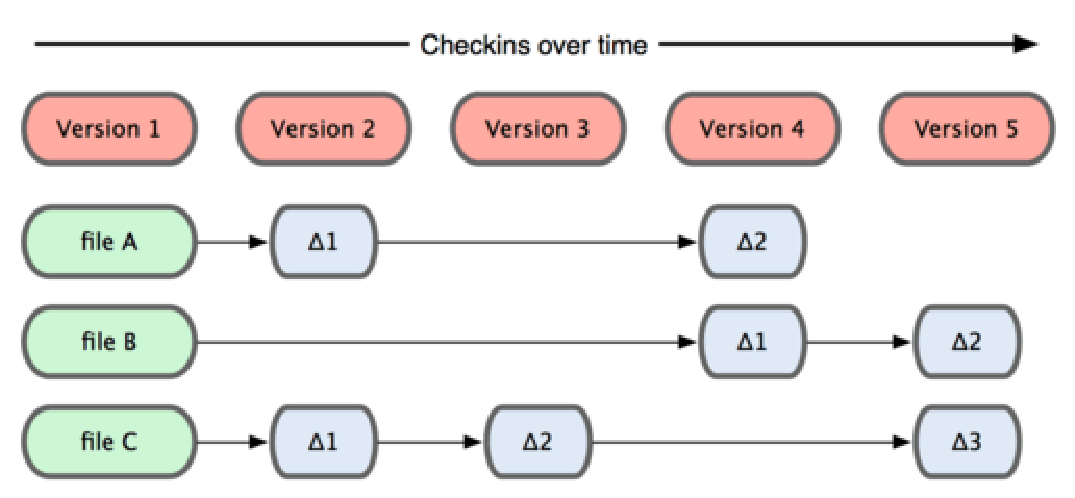
\includegraphics[width=1\linewidth]{other-scv}}
				\caption{Другие системы хранят данные как изменения к базовой версии для каждого файла.}
				\label{ris:other-scv}
			\end{figure}	
			\newpage
				Git не хранит свои данные в таком виде. Вместо этого Git считает хранимые данные набором слепков небольшой 						файловой системы. Каждый раз, когда вы фиксируете текущую версию проекта, Git, по сути, сохраняет слепок того, как 					выглядят все файлы проекта на текущий момент. Ради эффективности, если файл не менялся, Git не сохраняет файл снова, 				а делает ссылку на ранее сохранённый файл. То, как Git подходит к хранению данных, похоже на Рис.~\ref{ris:git}
			
			\begin{figure}[h!]
				\center{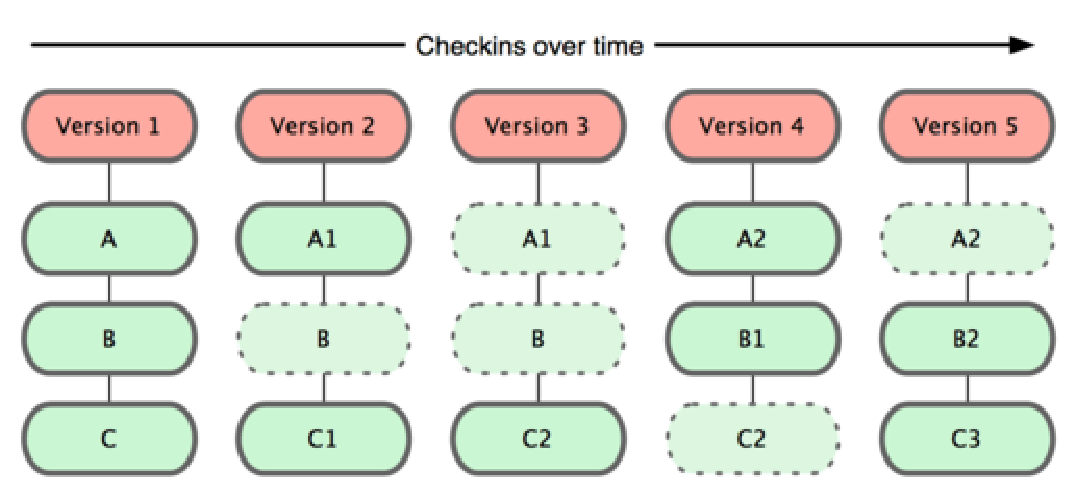
\includegraphics[width=1\linewidth]{git}}
				\caption{Git хранит данные как слепки состояний проекта во времени.}
				\label{ris:git}
			\end{figure}
			\newpage
				За счет этого, для большинства операций в Git нужны только локальные ресурсы и файлы. Что в свою очередь 						определяет два основных преимущества Git перед остальными СКВ.
			\begin{itemize}
	    		\item	Быстродействие. Поскольку вся история проекта хранится локально у вас на диске, большинство операций 							кажутся практически мгновенными(в отличии от централизованных системам, где практически на каждую операцию 							накладывается сетевая задержка).
	    		\item	Возможность работать(делать коммиты) без доступа к сети или VPN.
			\end{itemize}
			\newpage
			\subsubsection{Основные команды}
			В целом, следующая картинка (Рис.~\ref{ris:git-command}) наглядно демонстрирует основные команды Git, знание которых 			достаточно, чтобы начать им пользоваться.
			
		\begin{figure}[h]
			\center{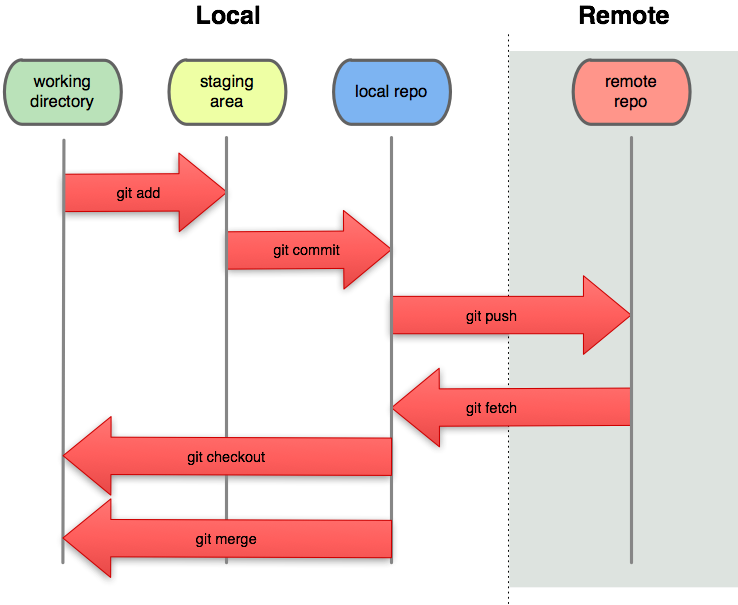
\includegraphics[width=0.75\linewidth]{git-command}}
			\caption{Основные команды при работе с Git.}
			\label{ris:git-command}
		\end{figure}
		\newpage
		\subsection{GitHub}
			\href{https://github.com/}{GitHub} — крупнейший веб-сервис для хостинга IT-проектов и их совместной разработки. 				Основан на системе контроля	версий Git и разработан на Ruby on Rails и Erlang компанией GitHub, Inc (ранее Logical 					Awesome).
			
			В ходе прохождения практики, на сайте GitHub была создана учетная запись ~\href{https://github.com/MorozovSD}					{MorozovSD}. В данной учетной записи был создан репозиторий ~\href{https://github.com/MorozovSD/Practice-2016}						{Practice-2016} по которому можно легко отследить процесс прохождения практической работы.
	\newpage
	\section{Паралельные вычисления}
		Т.к. практика предполагает не доскональное изучение параллельного программирования, а лишь сравнение функций замера 			времени в программах, работающих на основе парралельных вычислений, то данная глава носит более ознакомительных характер, 			содержащий тот минимум знаний, необходимый для работы с этой области.
		\subsection{Немножко теории}
		%Интуит Академия Microsoft: Параллельные вычисления и многопоточное программирование разделения компьютеров на три 						класса:	
			%Мультипроцессорные вычислительные комплексы - это компьютеры, обладающие множеством процессоров, работающих на общей 			памяти. В этот класс входит большинство продаваемых сегодня на рынке многоядерных компьютеров.

			%Мультикомпьютерные вычислительные комплексы - представляют множество компьютеров, соединенных высокоскоростными 				линиями связи. Каждый компьютер обладает собственной памятью и обменивается сообщениями с другими компьютерами системы 				для передачи данных. 
	
			Мультипрограммирование "--- параллельное выполнение нескольких программ. Мультипрограммирование позволяет уменьшить 			общее время их выполнения.
			
			Под параллельными вычислениями понимается параллельное выполнение одной и той же программы. Параллельные вычисления 			позволяют уменьшить время выполнения одной программы. Чаще всего, хороший последовательный алгоритм не является таковым 			для параллельного выполнения.(а параллельные алгоритмы могут не являться эффективными при работе с одним процессором), 				поэтому одна из задач паралельных вычислений это разработка эффективных алгоритмов, полностью использующие количество 				преподставленных процессоров. 
			
			Т.к. тема практики "--- измерение времени работы пареллельно работаящей программы, то необходимо получить оценку    			времени выполения программы одним процессором $T_1$  для идеализированного случая, когда число процессоров не 						ограничивается "--- $T_\infty$. А так же оценить верхнюю и нижнюю границы времени выполнения конечным число процессоров 			$T_p$\footnote{В отчете будут представленны только конечные формулы, без доказательств}.
						
		Для введенных характеристик очевидно следующее соотношение:

		\begin{equation}
			\label{eq:easy_attetude}
			T_\infty \le T_p \le T_1
		\end{equation}
			
		Для $T_p$ справедлива следующая оценка снизу:
			
		\begin{equation}
			\label{eq:lower_bound}
			T_p \ge \frac{T_1}{p}
		\end{equation}
			
		Для $T_p$ справедлива следующая оценка сверху:
			
		\begin{equation}
			\label{eq:upper_bound}
			T_p \le \frac{T_1}{p} + T_\infty
		\end{equation}
			
		Исходя из вышеперечисленных неравенств, неравенство(\ref{eq:easy_attetude}) может быть заменено более точным:
			
		\begin{equation}
			\label{eq:attetude}
			\frac{T_1}{p} \le T_p \le \frac{T_1}{p} + T_\infty
		\end{equation}
			
		\newpage

		На графике это выглядит следующим образом (Рис.~\ref{ris:graph_attetude}):
			
		\begin{figure}[h!]
			\center{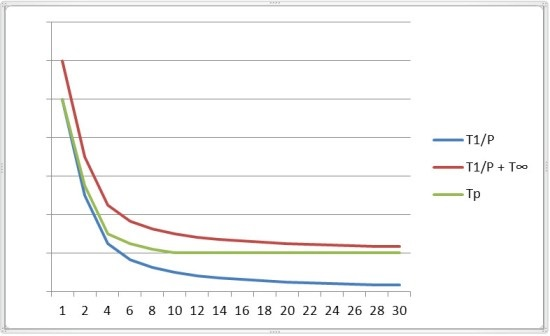
\includegraphics[width=1\linewidth]{graph_attetude}}
			\caption{Графическая интерпритация поведения функции $T_p$}
			\label{ris:graph_attetude}
		\end{figure}
						
			Очевидно, что при $p = 1$ графики функций $T_p$ и $\frac{T_1}{p}$ совпадают. Так же происходит совпадение графиков 				$T_p$ и $\frac{T_1}{p}+T_\infty$ при $p\to\infty$.
		\newpage
		\subsection{Характеристики параллельных вычислений}
			\subsubsection{Ускорение}
				Ускорение $S_p(n)$\footnote{Все вводимые характеристики рассматриваются как функции параметра $n$, 								характеризующего сложность решаемой задачи. Обычно $n$ понимается как объем входных данных.} определяют как 						отношение:
				
			\begin{equation}
				\label{eq:acceleration}
				S_p(n) = \frac{T_1(n)}{T_p(n)}
			\end{equation}			
				
				Интерпритировать данную формулу следует как отношение время наилучшего алгоритма, для которого достаточно одного 				процессора, и время наилучшего параллельного алгоритма, который может использовать $p$ имеющихся процессоров.				
				
			\subsubsection{Эффективность}
				Эффективность $E_p(n)$ определяют как отношение:
				
			\begin{equation}
				\label{eq:efficiency}
				E_p(n) = \frac{S_p(n)}{p}
			\end{equation}	

				При оптимальном ускорении\footnote{Оптимальное ускорение достигается когда $T_p = \frac{T_1}{p}$} эффективность 				равна 1. Если же эффективность существенно ниже 1, то часто число процессоров целесообразно уменьшить, используя 					их более эффективно. 
				
			\subsubsection{Упущенная эффективность}
				Мера неиспользованных возможностей - упущенной выгоды - $U(n)$, определяют следующим образом:
			
			\begin{equation}
				\label{eq:loss_of_efficiency}
				U(n) = \frac{T_p(n)}{T_{p_{opt}}} - 1
			\end{equation}
			
				Оптимальное время, которое можно достичь, используя $p$ процессоров, дается нижней оценкой для $T_p$, 							поэтому получаем:	

			\begin{equation}
				\label{eq:loss_of_efficiency_second}
				U(n) = p\frac{T_p(n)}{T_1} - 1
			\end{equation}
				
				Если для компьютера с p ядрами время решения задачи оптимально и сокращается в \~p раз в сравнении с решением 					задачи на одноядерном компьютере, то наши потери равны нулю, возможности компьютера полностью используются. Если же 				задача решается за время $T_1$ - столь же долго, как на одноядерном компьютере, то потери пропорциональны числу 					неиспользованных ядер.
				
		\subsection{Основные проблемы паралельного программирования}
		%http://www.intuit.ru/studies/courses/10554/1092/lecture/27087?page=6
		%http://www.intuit.ru/studies/courses/10554/1092/lecture/27089?page=2
		\subsection{Распарелеливание цикла}
		%http://www.intuit.ru/studies/courses/10554/1092/lecture/27091
	\newpage
	\section{Функции замера времени}
		%%Описывание разных функций замера времени
		\subsection{Принцип работы}
		%%Работают только в Windows		
		\subsection{Windows}
			\subsubsection{func1}
			\subsubsection{func2}
			\subsubsection{...}
		%%Работают только в Linux
		\subsection{Linux}
			\subsubsection{func4}
			\subsubsection{func5}
			\subsubsection{...}
	\newpage
		%%Работают и в Windows и в Linux
		\subsection{Кросплатформенные}
			\subsubsection{func7}
			\subsubsection{func8}
			\subsubsection{...}
		\subsection{Проблемы и сложности замеров времени \\ при параллельный вычислениях}
	\newpage
	\section{Практическая часть?}
		\subsection{Описание эксперементальной программы}
		\subsection{Результаты работы программы}
		%%Большая таблица сравнения развых функций замеров времени
		\subsection{Выводы}
		%%Сравнение функций
		%
		%http://www.intuit.ru/studies/courses/10554/1092/lecture/27087?page=2
	\newpage
	\section{Вывод по производственной практике}
	%%Вывод по всей работе
	\newpage
	\section{Список литературы}
	%% Буду делать в конце
	%%Ссылки, чтобы ничего не забыть
	%%http://mgena.chat.ru/latex/indru.html
	%%http://www.sbras.ru/win/docs/TeX/LaTex2e
	%%http://zns.susu.ru/IT/latex/literature/PartlS_LaTeX.pdf
	%%https://ru.sharelatex.com/learn/Page_size_and_margins
	%%http://elibrary.bsu.az/kitablar/1021.PDF
	%%http://zns.susu.ru/IT/latex/Marking/marking.html
	%%https://en.wikibooks.org/wiki/LaTeX/Title_Creation
	%%http://www.sbras.ru/win/docs/TeX/LaTex2e/Text_in_LaTeX.pdf
	%%TODO сделать красиво и по ГОСТ'у
\end{document}
